% !TeX root = ../report.tex
% !TeX spellcheck = en-US
% !TeX encoding = UTF-8


\section{SENSORS}\label{sec:sensors}

In the following section a variety of sensor types, their workings and useful applications, are presented. A 
selection is
made for sensor types that can be used underwater, in an environment which is deprived of a~\gls{acr-GPS} coverage.

The shortcomings and strength of the different sensor are often fused together with a complementary filter, where a 
mathematical filter is used to mix and merge the two values, or by use of a~\gls{gls-Kalman-filter} which is an 
algoritm, that uses a series of measurements observed over time, containing statistical noise and other inaccuracies 
and produces estimates of unknown variables that tend to be more precise than those based on a signle measurement 
alone. The following sections briefly describe the workings of an~\gls{gls-accelerometer}, 
~\gls{gls-gyroscope}~\gls{gls-magnetometer} and a~\gls{gls-pressure-sensor}, which will be used in 
Section~\ref{sec:KalmanRefinement}, where these sensors will be fused together with a~\gls{gls-Kalman-filter} to 
obtain an accurate heading and positioning system.

The sensors described in Section~\ref{sec:sensorstate} determine the state of a dredge bot; namely its orientation and
position. The sensors described in Section~\ref{sec:sensorenvironment} describes a variety of sensors which are needed
to gauge the environment.

\subsection{STATE SENSING}\label{sec:sensorstate}

In order for a dredge bot to perform its tasks it has to be aware of its state. As described in 
Section~\ref{sec:state representation}, the state vector \gls{sym-x_k} describes the position in a global reference 
frame and the orientation of the dredge bot itself. This state vector can be obtained using a fusion of multiple 
sensors, which are described below.

\subsubsection{INERTIAL MEASUREMENT UNIT}

\citet{leccadito_kalman_2013} describes \gls{acr-IMU} as a platform of sensors which output measurements of the
vehicle state, such as angular rates and accelerations. The sensors usually consist of a \gls{gls-gyroscope}, which
outputs angular rates about the three vehicle axes, and \gls{gls-accelerometer}, which output acceleration also along
each of the three axes. These sensors are sometimes complemented with a \gls{gls-magnetometer}, which measures the
strength of a magnetic field, like the one generated by the earth, along three axes.

\subsubsection{ACCELEROMETER}

There are many different types of \gls{acr-MEMS} based \glspl{gls-accelerometer}. The more expensive \gls{acr-MEMS} 
are laser and optical based, whilst cheaper models are piezoresistive, capacitive sensing and piezoelectric. 
\citet{leccadito_kalman_2013} describes the working of an \gls{gls-accelerometer} as follows; the sensor can be 
thought of as a ball in a box. If the \gls{gls-accelerometer} meter is still and there are no forces present, the 
sensor will measure \SI{0}{\meter\per\second\squared} on all three axes; the ball is suspended in air. If the sensor 
is suddenly moved, the ball will hit the wall with an opposing force compared to the movement. An acceleration can be
measured because of Newton's second law \( \gls{sym-F} = \gls{sym-m}  \gls{sym-a}  \).

In the scenario where there is no external forces present, the \gls{gls-accelerometer} would only measure the
acceleration of the opposite direction of movement, however, on earth there is the external force of gravity pulling on
the sensor. If the sensor is positioned on a flat surface with the z-axis aligned as up and down, x-axis left and right
and y-axis forward and back, gravity will always be in the negative z direction.

\begin{RoyalFigure}[!htb, label=fig:accelerometer_heading]{GRAVITATIONAL PULL ON MULTIPLE
AXES~\cite{leccadito_kalman_2013}}
    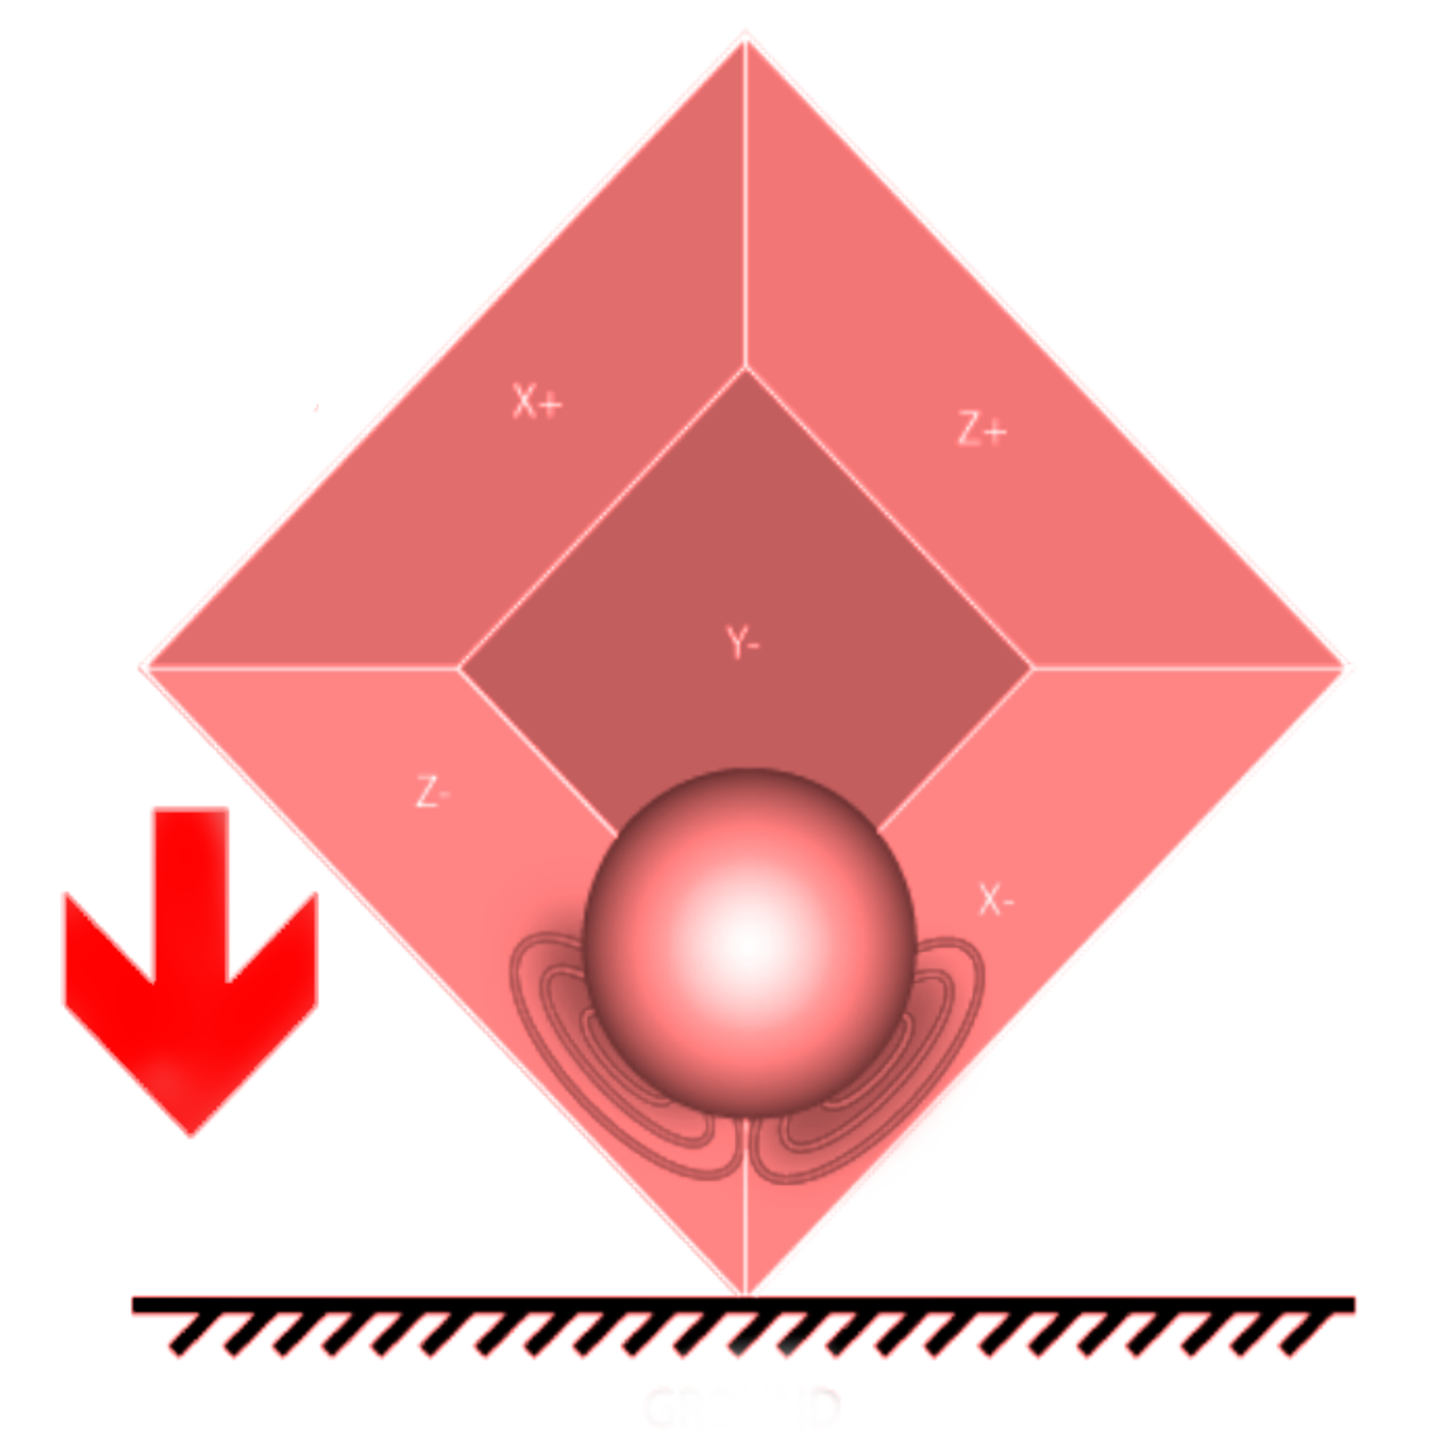
\includegraphics[height=5cm,trim=3 3 3 3,clip]{accelerometer.pdf}
\end{RoyalFigure}

Due to the gravitational pull, an \gls{gls-accelerometer} can be used to calculate the heading because the sensed 
acceleration is divided amongst the walls that the ball is in contact with, as is shown in 
figure~\ref{fig:accelerometer_heading}. These measurements can be directly computed into position or Euler angles 
roll \gls{sym-phi_imu} and pitch \gls{sym-theta_imu} using trigonometry which is shown in 
equation~\ref{eq:roll_and_pitch_accelerometer}. This allows the magnetometer to calculate a heading angle, which will
be described in section~\ref{sec:magnetometer}.

\begin{equation}
    \label{eq:roll_and_pitch_accelerometer}
    \left[ \begin{array}{c}
               \gls{sym-psi_imu}   \\
               \gls{sym-theta_imu} \\
               \gls{sym-phi_imu}
    \end{array} \right] =
    \left[\begin{array}{c}
              \arctan \left(-\frac{\gls{sym-a_y}}{\gls{sym-a_z}}\right)                                   \\
              \arcsin - \frac{\gls{sym-a_x}}{\sqrt{\gls{sym-a_x}^2 + \gls{sym-a_y}^2 + \gls{sym-a_z}^2 }} \\
              \text{Magnetometer Heading}
    \end{array}\right]
\end{equation}

Since acceleration can be integrated over time as velocity, which in turn can be integrated over time as a distance
travelled. \gls{gls-accelerometer}s can be used as a \gls{gls-dead-reckoning} device determining a location, with
respect to a starting position, in a \gls{acr-GPS} deprived environment. \citet{abyarjoo_implementing_2015} states that
the problem with accelerometers is that they measure both acceleration, due to the device's linear movement, and
acceleration due to the earth's gravity, which is pointing toward earth. Since it cannot distinguish between these two
accelerations, there is a need to separate gravity and motion acceleration by filtering. This is also described by
\citet{nistler_gravity_2011}, who further states that it should be clear that the measurement for a robotic vehicle on
an irregular terrain needs to be processed further if they are to be used in the robot \gls{gls-odometry} system.

Possible sources of error with \gls{acr-MEMS} \gls{gls-accelerometer}s are identified as effects of temperature and
discretization of an analog signal to its digital representation. \citet{abyarjoo_implementing_2015} observed no drift
of the signal but established that it contains a lot of noise. \citet{kownacki_optimization_2011} describes that a
\gls{gls-Kalman-filter} is a good candidate to filter the noise, using a gyroscope where the \gls{acr-ADC}
stores an obtained analog value as a digital representation. This is usually done with a resolution between \( 2^{10}
[bit] \) and \( 2^{16} [bit] \), resulting in a resolution of \( 1024 \), \( 2048 \) till \( 65536 \) but
discretization of a continuous signal inherently degrades it.

\subsubsection{GYROSCOPE}

\gls{gls-gyroscope} has been used for many years in navigation. They usually involve a spinning object, which is 
tilted perpendicular to the spin, allowing the angle of the reference surface to be measured. The angle is affected 
by tilting or rotating. \Gls{gls-gyroscope} which are usually used in electronics, are also classed as \gls{acr-MEMS}
. They are based on other principles such as a laser ring, which observes a phase shift between two laser being sent 
in a circular path. However, these sensor are expensive and the cheaper alternative is a \gls{gls-gyroscope} which 
uses a piezoelectric sensor that works because of a Coriolis effect coupled with vibrations.

\begin{RoyalFigure}[!htb, label=fig:gyro]{GYROSCOPE USING CORIALIS EFFECT~\cite{leccadito_kalman_2013}}
    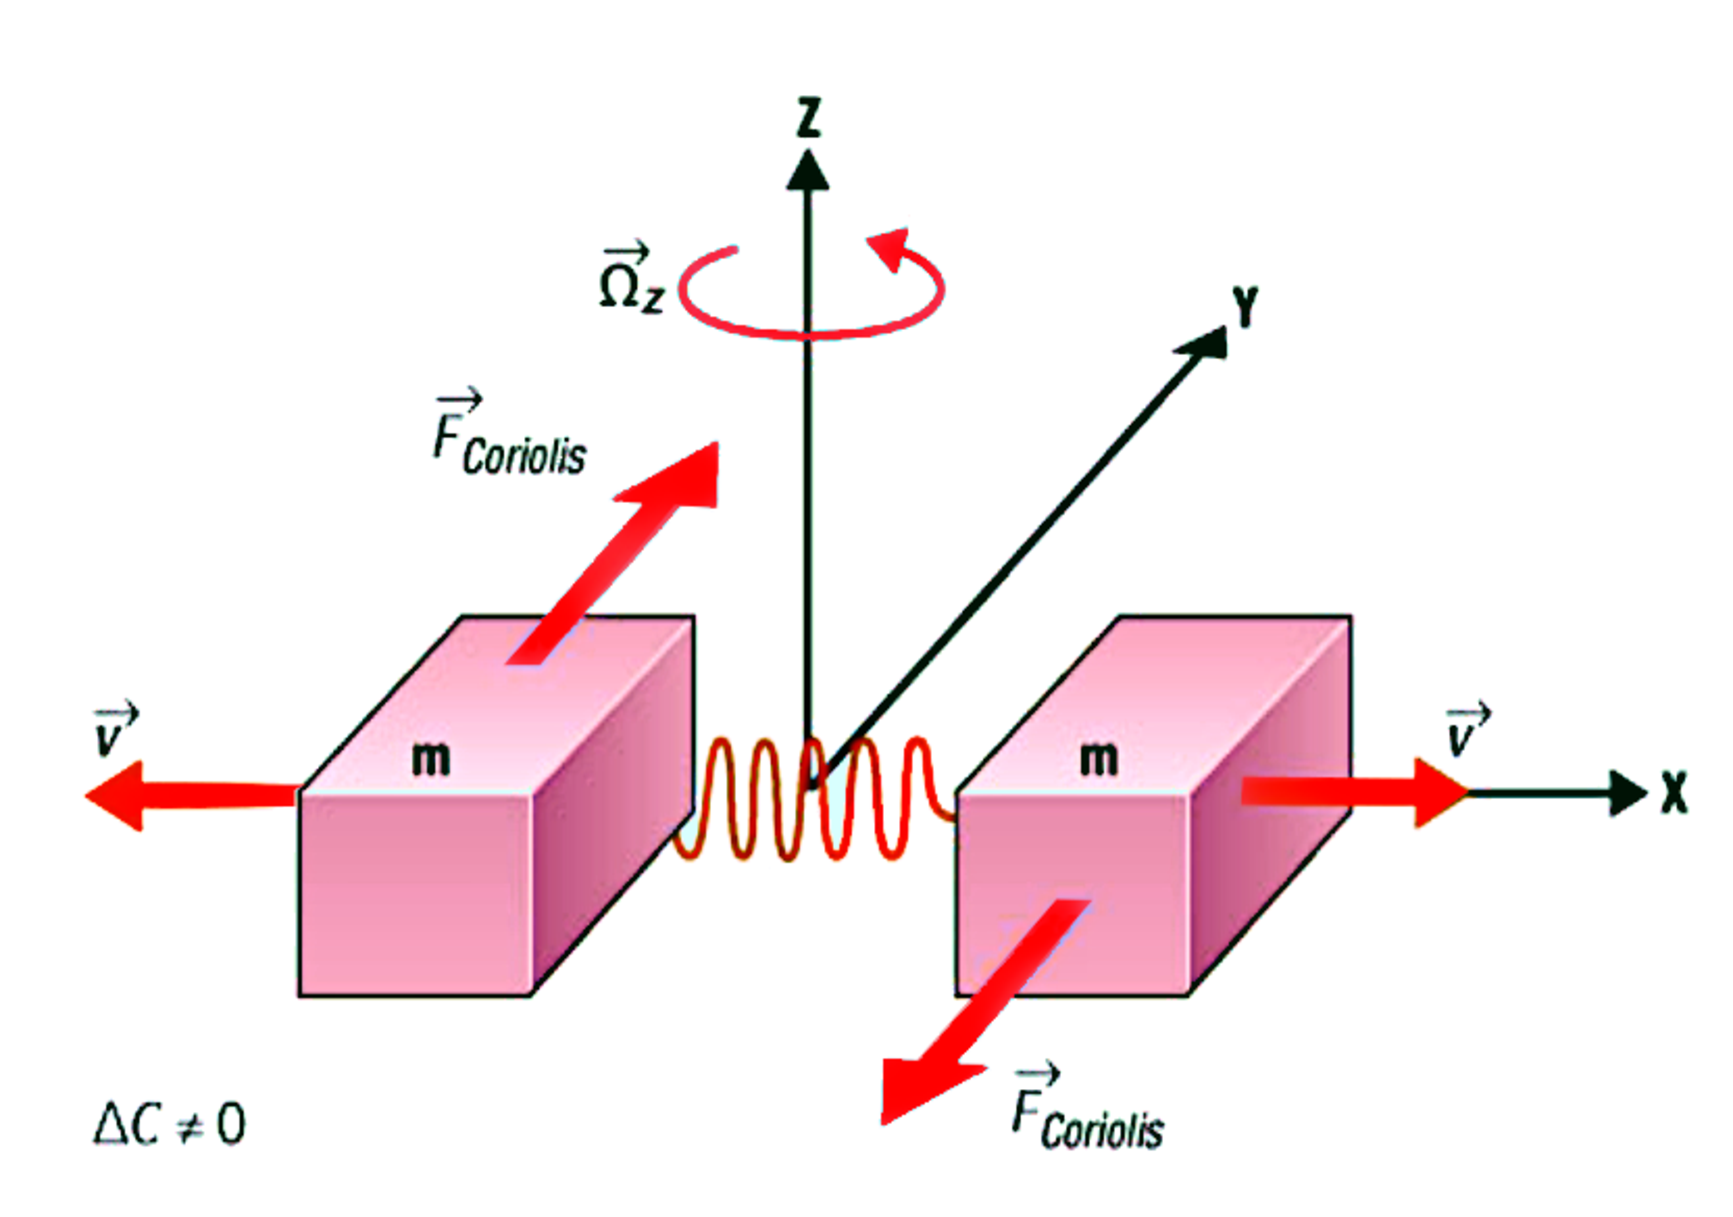
\includegraphics[height=5cm,trim=3 3 3 3,clip]{gyroscope.pdf}
\end{RoyalFigure}

\citet{leccadito_kalman_2013} tells that most \gls{acr-MEMS} \glspl{gls-gyroscope} are based on the tuning fork 
structure, where the \gls{gls-coriolis-effect} is used to measure \gls{sym-omega}, this is accomplished by two masses
oscillating in opposite directions. When a rotation is applied, the masses are affected by the Coriolis force and the
displacement is measured by a change in capacitance, as is shown in figure~\ref{fig:gyro}. The heading, at a certain 
axis, can be calculated using the \gls{gls-trapezoidal-rule} which is a technique for approximating the definite 
integral. Equation~\ref{eq:obtain_theta} illustrates how to obtain the current heading from a discrete sample set.

\begin{equation}
    \label{eq:obtain_theta}
    \gls{sym-theta}_n = \int_{\gls{sym-t}_{n-1}}^{\gls{sym-t}_n}\gls{sym-omega} \mathrm{d}x =
    \sum_{\gls{sym-t}_{n-1}}^{\gls{sym-t}_n}\gls{sym-omega} \mathrm{d}\gls{sym-t} \approx \gls{sym-theta}_{n-1} +
    \left(\gls{sym-t}_n - \gls{sym-t}_{n-1}\right)\left[\frac{\gls{sym-omega}(\gls{sym-t}_{n-1}) + \gls{sym-omega}
    (\gls{sym-t}_{n})}{2}\right]
\end{equation}

\citet{abyarjoo_implementing_2015} observed that the computed results drift over time. The explanation for this 
phenomenon is that the integration accumulates the noise over time and turns noise into the drift, which yields 
unacceptable results. Another source of drift is temperature related, \citet{feng_adaptive_2015} state that a 
\gls{gls-gyroscope} is sensitive to temperature variations, so the surrounding temperature variations lead to a bias 
drift of the gyroscope. Then, as an error of the angular velocity, the drift causes error accumulation in the 
orientations where this drift is not linear with temperature. Equation~\ref{eq:model_drift_gyro} shows the model of a
\gls{acr-MEMS} \gls{gls-gyroscope} drift, \gls{sym-omega_t} is the true angular velocity, but unknown and 
\gls{sym-B_d} is a slow changing component of the signal; this is the gyroscope drift. \gls{sym-n_s} is the 
stochastic component of a signal.

\begin{equation}
    \label{eq:model_drift_gyro}
    \gls{sym-omega} = \gls{sym-omega_t} + \gls{sym-B_d} + \gls{sym-n_s}
\end{equation}

\citet{abyarjoo_implementing_2015} further states that the slow chancing component of the \gls{gls-gyroscope} is not 
only related to the measured temperature of the \gls{acr-MEMS}, but also related to the temperature gradient of the 
surroundings. Because the temperature gradient and the rate of temperature variation have a linear relationship, the 
slow-chancing component \gls{sym-B_d} can be modelled, as shown in equation~\ref{eq:model_bd} \( a \), \( b \), and 
\( c \) are the parameters of the model \cite{wei_improved_2006} and \gls{sym-T} is the measured temperature of the 
\gls{gls-gyroscope} in \glsunit{sym-T} and \gls{sym-T_prime} is the rate of temperature variation in time.

\begin{equation}
    \label{eq:model_bd}
    \gls{sym-B_d} = a\gls{sym-T} + b\gls{sym-T_prime} + c
\end{equation}

Other sources of errors are the conversion from the generated analog signal to a digital representation. The
\gls{acr-ADC} in a \gls{acr-MEMS} stores the obtained analog value as a discrete digital representation with a certain
sequence of bits. This is usually done in \gls{gls-word} with a resolution between \( 2^{10} [bit] \) and \( 2^{16}
[bit] \), resulting in a resolution of \( 1024 \), \( 2048 \) till \( 65536 \) which should be stored in two
registries. Discretization of a continuous signal inherently degrades it.

\subsubsection{MAGNETOMETER}\label{sec:magnetometer}

A \gls{gls-magnetometer} measures the strength of a magnetic field. A \gls{acr-MEMS} \gls{gls-magnetometer} operates 
by detecting the effects of the \gls{gls-lorentz-force} resulting in a change in voltage or resonant frequency which 
can be measured electronically. \citet{leccadito_kalman_2013} who explains that a \gls{gls-magnetometer} coupled with
an \gls{gls-accelerometer} can effectively calculate a heading angle. This is further explained by 
\citet{konvalin_technical_2008} whom explain that raw magnetometer measurements cannot be used to calculate the 
heading angle due to the decrease in sensitivity as elevation and bank angles increase, introducing error. In order 
to obtain the correct heading, a rotation must first be applied removing the bank angle, after which removes the 
pitch angle. This can be obtained by equation~\ref{eq:roll_and_pitch_accelerometer} where the heading, or yaw 
\gls{sym-psi_imu} can be calculated following equations~\ref{eq:x_h} through~\ref{eq:theta_imu} where \gls{sym-x_m}, 
\gls{sym-y_m} and \gls{sym-z_m} are the raw \gls{gls-magnetometer} values.

\begin{equation}
    \label{eq:x_h}
    \gls{sym-x_h} = \gls{sym-x_m} \cos \gls{sym-theta_imu} + \gls{sym-z_m} \sin \gls{sym-theta_imu}
\end{equation}

\begin{equation}
    \label{eq:yh}
    \gls{sym-y_h} = \gls{sym-x_m} \sin \gls{sym-phi_imu} \sin \gls{sym-theta_imu} + \gls{sym-y_m} \cos
    \gls{sym-phi_imu} - \gls{sym-z_m} \sin \gls{sym-phi_imu} \cos \gls{sym-theta_imu}
\end{equation}

\begin{equation}
    \label{eq:theta_imu}
    \gls{sym-phi_imu}(\gls{sym-y_h},\gls{sym-x_h}) = \left[\begin{array}{ll}
                                                               \arctan\left
                                                               (\frac{\gls{sym-y_h}}{\gls{sym-x_h}}\right) &
                                                               \text{if } \gls{sym-x_h} > 0 \\
                                                               \arctan\left
                                                               (\frac{\gls{sym-y_h}}{\gls{sym-x_h}}\right) + \pi &
                                                               \text{if } \gls{sym-x_h} < 0, \gls{sym-y_h} \geq 0 \\
                                                               \arctan\left
                                                               (\frac{\gls{sym-y_h}}{\gls{sym-x_h}}\right) - \pi &
                                                               \text{if } \gls{sym-x_h} < 0, \gls{sym-y_h} < 0 \\
                                                               +\frac{1}{2} \pi
                                                               & \text{if } \gls{sym-x_h} = 0, \gls{sym-y_h} > 0 \\
                                                               -\frac{1}{2} \pi
                                                               & \text{if } \gls{sym-x_h} = 0, \gls{sym-y_h} < 0 \\
                                                               \text{undef}
                                                               & \text{if } \gls{sym-x_h} = 0, \gls{sym-y_h} = 0
    \end{array}\right]
\end{equation}

The main sources of error using a \gls{gls-magnetometer} are distortions of the earth's magnetic field, which can be 
classified in two categories: soft and hard iron. \Gls{gls-hard-iron} distortions can be described as a constant 
additive disturbance in the magnetic field of the magnetometer which can be created by ferrous materials around the 
sensors such as the construction of a crawler and the casing of the electronics and hydraulics. This can create its 
own magnetic field and adds to the sensor's magnetic fields and is in constant position relative to the sensor. 
According to \citet{leccadito_kalman_2013}, such a distortion is constant and can be eliminated by a constant offset 
or bias. To eliminate the offset equation~\ref{eq:offset} can be used. Where \gls{sym-m_vec} is the raw 
magnetometer vector and \gls{sym-m_hi} is the hard iron adjusted vector. This is offset from centre obtained by 
averaging the minimum and maximum value in \( n \) calibration values obtained by rotating the sensor in the iron 
casing. Since this value will be constant, it can be stored in memory.

\begin{equation}
    \gls{sym-m_vec} =
    \left[\begin{array}{c}
              \gls{sym-x_m} \\
              \gls{sym-y_m} \\
              \gls{sym-z_m}
    \end{array}\right]
\end{equation}

\begin{equation}
    \label{eq:offset}
    \gls{sym-m_hi} = \gls{sym-m_vec} - \frac{\min(\gls{sym-m_vec})_n + \max(\gls{sym-m_vec})_n}{2}
\end{equation}

\Gls{gls-soft-iron} distortions are different from \gls{gls-hard-iron} disturbances since they don't necessarily
generate their own magnetic field. \citet{leccadito_kalman_2013} describes that soft iron effects on the sensor are
determined by the orientation of the materials, and it's usually a perturbation of a circular magnetic field to an
ellipse. Calculating the \gls{gls-soft-iron} distortion is computationally more expensive than the \gls{gls-hard-iron}
elimination.

\begin{RoyalFigure}[!htb, label=fig:ellipse]{SOFT IRON DISTORTION~\cite{konvalin_technical_2008}}
    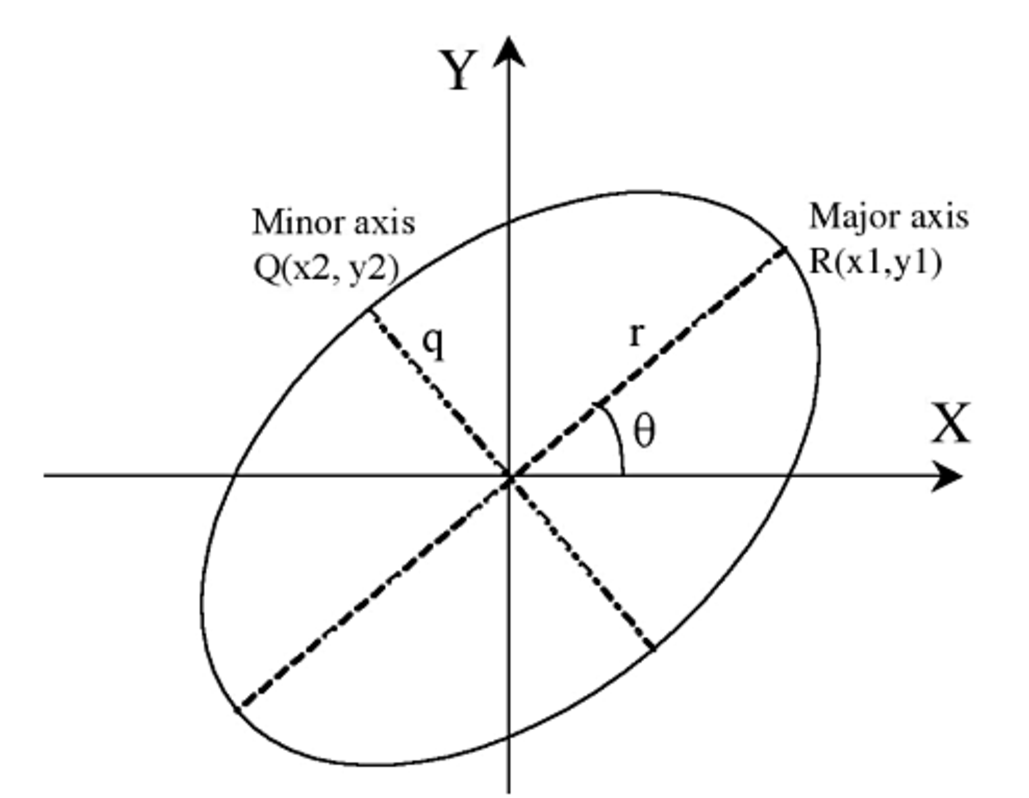
\includegraphics[height=5cm,trim=3 3 3 3,clip]{softiron.pdf}
\end{RoyalFigure}

it's assumed that tilt compensation (eq.~\ref{eq:theta_imu}) and \gls{gls-hard-iron} offset (eq.~\ref{eq:offset}) are
already performed at this stage and that the centre of the ellipse is positioned at point \( (0,0) \), which is drawn
in figure~\ref{fig:ellipse}. The first step is to calculate the magnitude of each point on the ellipse and find the 
smallest and greatest value, using equation~\ref{eq:ellipse_max} and~\ref{eq:ellipse_min}. The y-index of the 
greatest magnitude should be stored in \gls{sym-y_1}, which together, can be used to calculated \gls{sym-theta_si}, 
as is shown in equation~\ref{eq:theta_ellipse}. By scaling and rotating the \gls{gls-hard-iron} \gls{sym-m_hi} 
vector, a correct heading \gls{sym-m_si} can be calculated, which is shown in equation~\ref{eq:correct heading}.

\begin{equation}
    \label{eq:ellipse_max}
    \gls{sym-r_si} = \max \left(\sqrt{x_n^2 + y_n^2}\right)
\end{equation}

\begin{equation}
    \label{eq:ellipse_min}
    \gls{sym-q_si} = \min \left(\sqrt{x_n^2 + y_n^2}\right)
\end{equation}

\begin{equation}
    \label{eq:theta_ellipse}
    \gls{sym-theta_si} = \arcsin\left(\frac{\gls{sym-y_1}}{\gls{sym-r_si}}\right)
\end{equation}

\begin{equation}
    \label{eq:correct heading}
    \gls{sym-m_si} = \frac{\gls{sym-q_si}}{\gls{sym-r_si}} \left[\begin{array}{ccc}
                                                                     \cos \gls{sym-theta_si} & \sin
                                                                     \gls{sym-theta_si} & 0 \\
                                                                     -\sin \gls{sym-theta_si} & \cos
                                                                     \gls{sym-theta_si} & 0 \\
                                                                     0 & 0
                                                                     & 1
    \end{array}\right] \gls{sym-m_hi}
\end{equation}

\subsubsection{PRESSURE SENSOR}\label{sec:pressure sensor}

\citet{white_fluid_2011} describes a fluid pressure \gls{sym-p} as the normal shear stress on any plane through a 
fluid element at rest is an infinitesimal point property, which is taken positive for compression, by convention. 
This can be described by equation~\ref{eq:depth}. Here \gls{sym-p} is the pressure at a certain depth, which is 
comprised of the specific weight of water \( \gls{sym-gamma_w}(\gls{sym-T}) \) as a function of temperature, and the 
total mass of water on top of that point \gls{sym-z}.

\begin{equation}
    \label{eq:depth}
    \gls{sym-p} = \gls{sym-p_a} - \gls{sym-gamma_w}(\gls{sym-T}) \gls{sym-z}
\end{equation}

Since pressure is a function of \gls{sym-gamma_w} special consideration regarding the impact of soil disturbance due to
dredging activities in water, has to be made. The specific weight of the water column above the sensor changes
when sediment is mixed with water above the pressure sensor. \gls{acr-MTI} dredging specialists Dr.~ir.~van Wijk and
ir.~Hoftsra both estimate that the disturbed sediment won't drift higher than \SI{2}{\metre} for a sediment with an
\emph{in situ} specific weight of \( \gls{sym-gamma_sw} = \SI{1400}{\N\per\cubic\meter} \). That mixture will in all
likelihood have a specific weight of \( \gls{sym-gamma_m} = \SI{1200}{\N\per\cubic\meter} \) because the specific
weight of water is \( \gls{sym-gamma_w} = \SI{1000}{\N\per\cubic\meter} \). The error when calculating depth with a
\gls{gls-pressure-sensor} is dependent on the position of the sensor with regards to the bottom.

Using equation~\ref{eq:position pressure error}, \gls{sym-Delta_p} is the pressure difference between the specific 
weight of a column of water \gls{sym-gamma_w} compared with a column of water and sediment  \gls{sym-gamma_m}  of a 
certain height \gls{sym-z_p}. The specific weight consists of the density of a fluid \gls{sym-rho_w} for water or 
\gls{sym-rho_m} for mixture multiplied with a gravitational acceleration vector \gls{sym-g}. When the allowed 
\gls{sym-z_epsilon} is known. A height for the pressure sensor, with regards to the top fluid column can be obtained.
it's estimated that an acceptable error in depth readings is \SI{200}{\mm}, when using equation~\ref{eq:position 
pressure error} gives a minimum sensor height of \SI{1.9}{\meter} from the soil bed. This indicates that the sensor 
should be placed at the top of a dredge bot, away from the disturbance source.

\begin{equation}
    \label{eq:position pressure error}
    \left.
    \begin{array}{lcl}
        \Delta \gls{sym-p}  & = & \left(\gls{sym-gamma_w}-\gls{sym-gamma_m} \right)\gls{sym-z_p} \\[0.5em]
        \gls{sym-gamma_w}   & = & \gls{sym-rho_w}\gls{sym-g} \\ [0.5em]
        \gls{sym-gamma_m}   & = & \gls{sym-rho_m}\gls{sym-g} \\ [0.5em]
        \gls{sym-z_epsilon} & = & \frac{\Delta \gls{sym-p}}{\gls{sym-gamma_w}}
    \end{array}
    \right\} \gls{sym-z_epsilon} = \frac{-\left(\gls{sym-rho_m}-\gls{sym-rho_w}\right)\gls{sym-z_p}}{\gls{sym-rho_w}}
    \Longrightarrow \gls{sym-z_p} = \frac{\gls{sym-z_epsilon} \gls{sym-rho_w}}{\gls{sym-rho_m} - \gls{sym-rho_w}}
\end{equation}

\noindent Three types of pressure measurements are usually performed, according to \citet{webster_measurement_1999}:

\begin{RoyalTable}{X[2,l,m] X[4,l,m]}
    \RoyalHeader{TYPE|DESCRIPTION}
    \RoyalRow{Absolute pressure|Where the pressure is measured against an perfect vacuum where pressure is zero.}
    \RoyalRow{Gage pressure|Is the pressure difference between the point of measurement and the ambient.}
    \RoyalRow{Differential pressure|Is the pressure difference between two points, one of which is chosen to be the
    reference. In reality, both pressures can vary, but only the pressure difference is of interest here.}
\end{RoyalTable}

Since pressure is defined as the force per unit area, the most direct way of measuring pressure is to isolate an area on
an elastic mechanical element for the force to act on. The deformation of the sensing element produces displacements and
strains that can be precisely sensed to give a calibrated measurement of the pressure~\cite{webster_measurement_1999}.

\begin{RoyalNote}{SCOPE}
    Although there are a multitude of pressure sensing techniques, such as: seals, snubbers, bellow, bourdon, helical,
    diaphragm, differential, electronic and manometers. This research will focus on diaphragm and electronic pressure
    sensors, since these are commonly used throughout the industry and easily integrated in a crawler. Where the focus
    lies on behavior and characteristics.
\end{RoyalNote}

Pressure sensors that depend on deflection of a diaphragm have been used for centuries, the last few decades the elastic
hysteresis, friction and drift effects have been reduced to \SI{\pm 0.1}{\percent}. This is mainly due to the use of a
microprocessor, which applies memorized non-linearity corrections~\cite{liptak_instrument_2003}.

Detection methods are usually capacitive \gls{gls-pressure-sensor}s, which are highly accurate (better than
\SI{0.1}{\percent}) and can cover a high pressure range, from nearly vacuum \SIrange{1e-1}{1e7}{\pascal}. These sensors
rest on the principle, where a metal or silicon diaphragm serves as the pressure sensing element and is regarded as one
electrode of a capacitor. The other electrode is stationary and usually consists of a deposited metal layer on a ceramic
or glass substrate. When a pressure is applied the diaphragm deforms and the changes in between electrodes is changed
which results in a change in capacitance.

Where an alternative are the piezoresistive \gls{gls-pressure-sensor}s, which are the most common type of
\gls{gls-pressure-sensor} in use. These sensors measure the pressure by measuring the change in electric resistance of a
material when stresses or strains are applied. Both \citet{webster_measurement_1999} and \citet{liptak_instrument_2003}
state that semiconductor, such as silicon and germanium, are by far the most appealing sensing elements in this type of
sensor. The most attractive characteristic of semiconductors is their sensitivity, which is close to \( 100 \) times
greater than that of metallic wires.

\subsection{EXTERNAL SENSOR}\label{sec:sensorenvironment}

A crawler needs to be aware of its surroundings; It needs to sense how far objects and landmarks are in respect to its
own position and orientation. Awareness of its environment can be used to minimize \gls{gls-dead-reckoning} drift,
defined the work area and help avoid collisions.

\begin{RoyalNote}{SCOPE}
    Although there are multiple examples of \gls{acr-AUV}s that make use of \gls{acr-EMW}, light or computer vision to
    help them sense its environment, these are deemed not usable for a crawler. \gls{acr-EMW} has a limited range in
    salt water environments (discussed in Section~\ref{sec:em}), light will scatter due to diffraction created by floating
    floating sand particles and computer vision can be problematic due to limited light sources and low contrast
    conditions. Which is also a result of floating sand particles. The focus of this research will therefor lie on
    acoustic sensing.
\end{RoyalNote}
\clearpage